\documentclass{article}

\usepackage{geometry}
\usepackage{makecell}
\usepackage{array}
\usepackage{multicol}
\usepackage{setspace}
\usepackage{changepage}
\usepackage{booktabs}
\usepackage{graphicx}
\usepackage[explicit]{titlesec}
\usepackage{hyperref}
\usepackage{cprotect}
\usepackage{float}
\newcolumntype{?}{!{\vrule width 1pt}}
\newcommand{\paragraphlb}[1]{\paragraph{#1}\mbox{}\\}
\renewcommand{\contentsname}{Inhaltsverzeichnis:}
\renewcommand\theadalign{tl}
\setstretch{1.10}
\setlength{\parindent}{0pt}

\titleformat{\section}
  {\normalfont\Large\bfseries}{\thesection}{1em}{\hyperlink{sec-\thesection}{#1}
\addtocontents{toc}{\protect\hypertarget{sec-\thesection}{}}}
\titleformat{name=\section,numberless}
  {\normalfont\Large\bfseries}{}{0pt}{#1}

\titleformat{\subsection}
  {\normalfont\large\bfseries}{\thesubsection}{1em}{\hyperlink{subsec-\thesubsection}{#1}
\addtocontents{toc}{\protect\hypertarget{subsec-\thesubsection}{}}}
\titleformat{name=\subsection,numberless}
  {\normalfont\large\bfseries}{\thesubsection}{0pt}{#1}

\hypersetup{
    colorlinks,
    citecolor=black,
    filecolor=black,
    linkcolor=black,
    urlcolor=black
}

\geometry{top=12mm, left=1cm, right=2cm}
\title{\vspace{-1cm}Konfigurationsmanagement 1}
\author{Andreas Hofer}

\begin{document}
	\maketitle
	\tableofcontents
	\newpage
	Configuration management is based on the concept of continuous integration, a process in which software is improved upon over a longer period of time in order to improve, further and enhance its functionality as well as documenting the process. In addition it also concerns itself with delivering executables in many different environments. \\
	This lecture is structured in six sections:
	\begin{enumerate}
		\item{Documentation}
		\begin{itemize}
			\item{Informing the user or other maintainers about the program's functions or requirements}
		\end{itemize}
		\item{Project Structure and Layout}
		\begin{itemize}
			\item{[TODO] Project Structure}
		\end{itemize}
		\item{Version Management}
		\begin{itemize}
			\item{Managing different iterations of projects as well as being able to recover from}
		\end{itemize}
		\item{Building}
		\begin{itemize}
			\item{The automatic creation of executables and figuring out issues with the build process}
		\end{itemize}
		\item{Testing}
		\begin{itemize}
			\item{Automatically testing components in order to figure out problems quickly}
		\end{itemize}
		\item{Releasing}
		\begin{itemize}
			\item{Releasing }
		\end{itemize}
	\end{enumerate}
	\section{Documentation}
	Documentation serves to inform the user or another programmer about the functions, how to maintain or change the poject, or how to use it. One of the most common ways to implement that is the so-called README file. \\
	\subsection{README}
	READMEs are usually very small text files added in the top-most folder of the application which briefly explains how to use it. It is generally a good idea to create the README \textit{before} starting with the project. A popular format to write them in is \textit{Markdown}, a markup language. \\
	Markup Languages are a family of languages which are used to format text in a specific way. HTML (Hypertext Markup Language) is one of these languages but tends to be difficult to use quickly, when all you want is to write how to use a program. Latex too is a markup language but isn't too handy without compiling it to a pdf, at which point it cannot be changed anymore. \\
	Because of that Markdown (MD) is an ideal format to write documentation in, since it only uses minimal formatting to \textit{italise} or \textbf{bold} text.\\
	\subsubsection{Markdown Syntax}
	Some formatting rules for Markdown are:
	\begin{itemize}
		\item{\textit{italic text} is created using *single asterisks*}
		\item{\textbf{bold text} is created using a **double asterisk**}
		\item{Headers can be created in two different ways:}
		\begin{itemize}
			\item{Either by adding pound signs to the left of the title. The higher the number of pound signs, the lower the header. \verb|# Title 1 / ## Title 2|}
			\item{Alternatively the first and second header can be created using either = or - in a new line beneath it respectively.}
			\item{\texttt{Title 1}}
			\item[]{\texttt{======}}
			\item{\texttt{Title 2}}
			\item[]{\texttt{------}}
		\end{itemize}
		\item{Headers are signified by using the pound sign \#, while depending on the number of consecutive signs to go further down in the hierarchy}
		\item{In order to create lists, there are several options}
		\begin{itemize}
			\item{For an unordered list, add one asterisk to the left of the *item}
			\item{For an ordered list, add the number to the left of the 1. item}
		\end{itemize}
		\item{In order to use any of these special characters within the text you can add a backslash before it (Escaping it) \\*}
	\end{itemize}

	\newpage
	\subsection{Cheatsheet}
	\begin{tabular}{| l | l | l |}
		\toprule
		Name & Markdown & Result \\ \midrule
		italic & *italic* & \textit{italic} \\ \hline
		bold & **bold** & \textbf{bold} \\ \hline
		
		\bottomrule
	\end{tabular}
	\newpage
	\section{Project Structure}
	With increasing project size, the amount of loose files can become hard to keep track of. To make that easier, it is a good idea to group files based on their purpose within the project. IDEs tend to automatically create grouping folders so it is not all just lying in one folder.
	\subsection{Maven}
	One system to help with this is \textbf{Maven} which helps manage Java projects across its lifecycle. It provides a uniform build system by standardising the process through the so-called \textit{pom.xml} (Project Object Model). It includes basic information about the project as well as build and environment settings. It for example automatically downloads dependencies listed in it so the user doesn't have to manage it. This may seem overkill for smaller projects but it becomes essential for larger projects. Often different components require different versions of libraries and management files help maintain these dependencies. In addition it also enables the maintainer to share the pom.xml file and ideally immediately have the build system set up the environment. Another feature is automated testing, where the system can automate running and evaluating all available unit tests. \\
	Maven achieves this structure by using predefined folders for specific project components so it is uniform between all Maven projects. For example it fully separates build and test environments, grouping these in different folders.
	\section{Versioning}
	Versioning helps with maintaining a clear structure for logging changes on the project. So whenever anything is added, removed or changed, the versioning system will log it. It also helps to return to a previous version should an error have emerged in a later version. This is not too relevant for small projects but large enterprise systems tend to have thousands over thousands lines of code with many hundred classes all interacting with each other. Maybe some of the maintainers are no longer part of the organisation or working somewhere else but with versioning you can see who made which changes. In addition it prevents careless changes to production code by requiring Pull Requests (Requests to change the repository code) to be confirmed by another person. \\
	Versioning systems can also help more efficiently comparing different versions by visually adjusting the code to show where something was added or removed. These versions can also be commented to add context to a change outside of comments within the code.
	\subsection{Types of Versioning}
	There are three kinds of versioning systems:
	\begin{itemize}
		\item{Local}
		\begin{itemize}
			\item{All versioning is exclusively stored on your computer preventing access from other people}
		\end{itemize}
		\item{Centralised}
		\begin{itemize}
			\item{Code is saved on a single server which multiple people can access and change}
		\end{itemize}
		\item{Distributed}
		\begin{itemize}
			\item{Each server and user has a full copy of the code}
			\item{Any changes are distributed to all users}
		\end{itemize}
	\end{itemize}
	\subsubsection{Local}
	Local versioning software is extremely easy to set up since all of the changes are only ever added to your own hard drive. It is very fast, since you have direct physical access to the medium and you also do not need to worry about security. \\
	As a disadvantage it is relatively difficult to cooperate with other people unless they come to your location. It is also not save from spontaneous data loss like a hard drive malfunction.
	\subsubsection{Centralised}
	In a centralised solution all the versions are only saved on a central server. Users tend to only use the version they are currently working on without having access to the entire version history. These systems allow for collaboration while being relatively easy to maintain since they only require a single server. But this single server is also a single point of failure and data loss can lead to a loss of most of the data. Since the code is only saved on the server, all access has to go through it as well, making access relatively slow.
	\subsubsection{Distributed}
	When each server and user maintains a full copy of the versions, a user has a lot more flexibility when making changes. Since everybody has all of the data you can make changes while offline and only synchronise when needed, upon which everybody receives the new version. \\
	This system is very robust since it has no single point of failure and upon data loss, there is a good chance that another user can use their own copy as a backup. But it is relatively data hungry sinc each user has everything available.
	\section{Git}
	The most commonly used versioning tool today is Git. It was developed by Linus Torvalds, creator of Linux, in order to make it easier to collaborate in its maintenance. Git changes the old approach of versioning systems to only save the changes from the previous version and instead saves a new version of a branch in its entirety. This change was made because large projects with hundreds of thousands of commits became painfully slow to figure out the newest version since it first had to calculate it based on all previous changes. This also made it possible to more easily branch away from the main version, which before that was slow and expensive to use. Git also calculates a checksum of each commit in order to preserve the integrity of this version and making data manipulation nearly impossible.
	\subsection{Stages}
	Within Git files can be in three stages:
	\begin{itemize}
		\item{Modified}
		\begin{itemize}
			\item{An already existing file had been modified}
		\end{itemize}
		\item{Staged}
		\begin{itemize}
			\item{A new or modified file is added to be committed}
		\end{itemize}
		\item{Committed}
		\begin{itemize}
			\item{Files have been committed and added to the versioning}
		\end{itemize}
	\end{itemize}
	\subsection{Recording Changes}
	Git additionally tracks the states files are in.
	\begin{itemize}
		\item{Untracked}
		\begin{itemize}
			\item{Files which have not (yet) been added to the versioning.}
			\item{Can be added by using \texttt{git add}}
		\end{itemize}
		\item{Unmodified}
		\begin{itemize}
			\item{Files which have been committed are changed to unmodified}
		\end{itemize}
		\item{Modified}
		\begin{itemize}
			\item{Files which have been changed are saved as modified until they are committed again}
		\end{itemize}
		\item{Staged}
		\begin{itemize}
			\item{Modified or new files which are set to be committed}
		\end{itemize}
	\end{itemize}
	\begin{figure}[H]
	\centering
	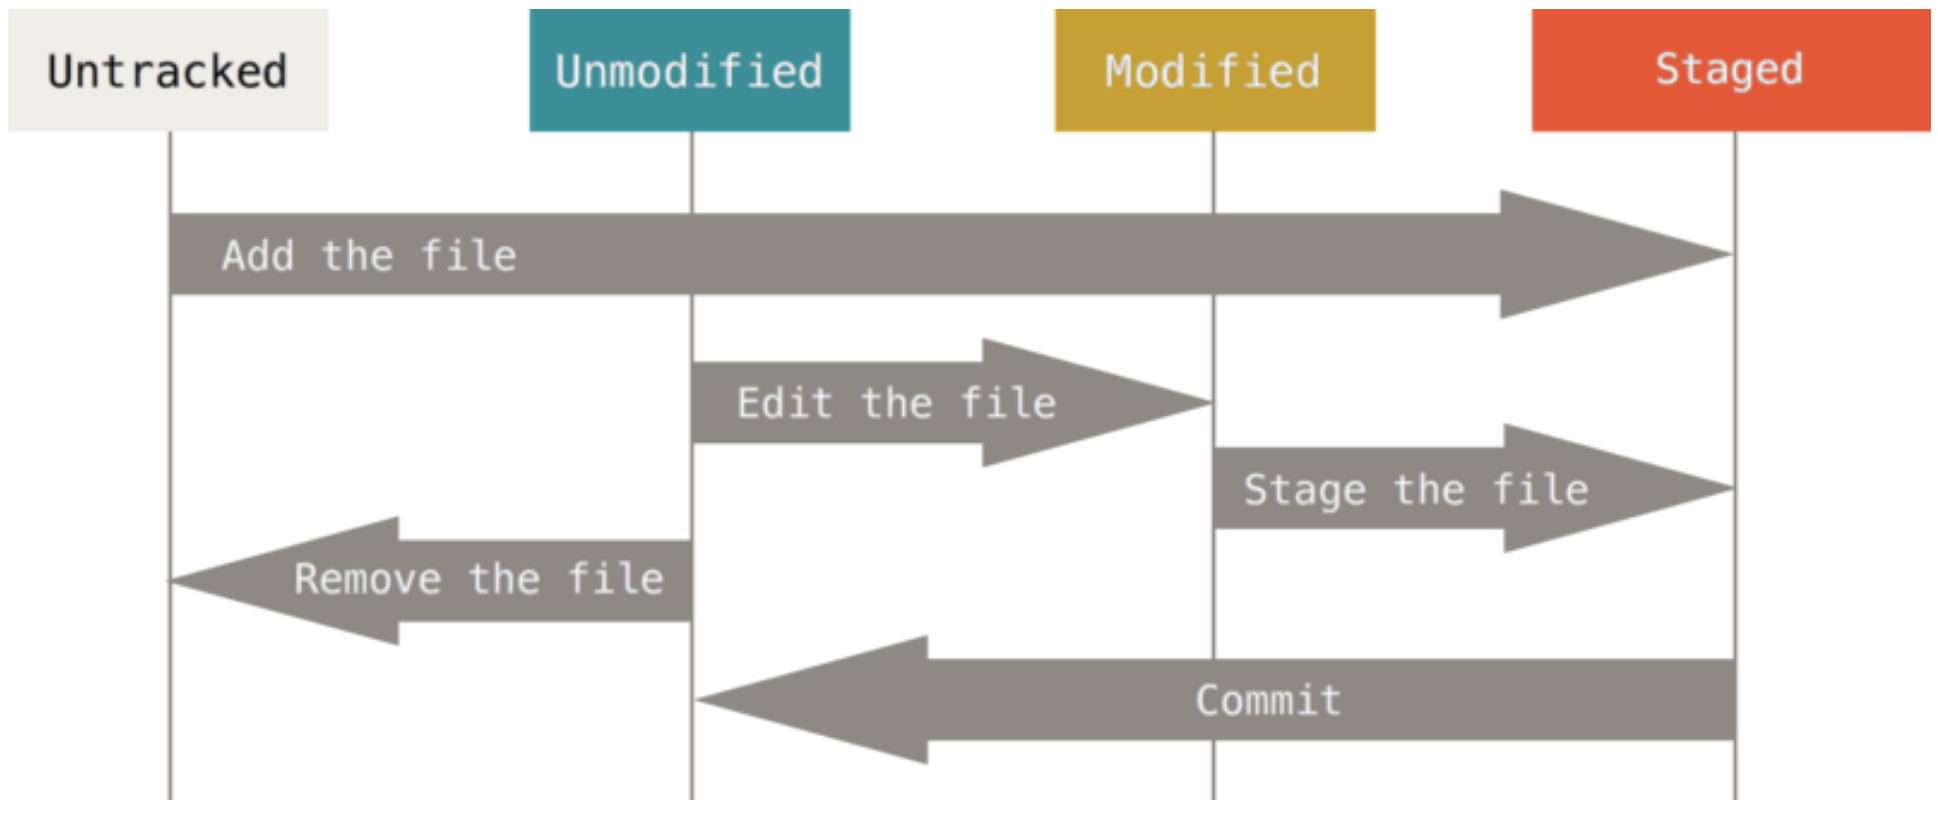
\includegraphics[scale=0.4]{Bilder/git_states.png}
	\caption{Different states of files in Git}
	\end{figure}
	
	\subsection{Commands}
	Git by default is a Command Line Interface (CLI) so it also uses commands to access its features. Some of its most important commands are:
	\subsubsection{\texttt{init}}
	\texttt{Init} initialises a new git repository in the current folder and automatically adds the main branch.
	\texttt{git init -> Creates new Git repository}
	\subsubsection{\texttt{status}}
	\texttt{status} shows the current state of the repository, informing you which branch you are currently on and all changes currently set to be committed. (Achieved through \texttt{add}) \\
	\texttt{git status -> Prints the branch status}
	\subsubsection{\texttt{add}}
	\texttt{Add} adds all specified files found in the folder. It supports batching commands so you can use either '*' or '.' to add all available files. \\
	\texttt{git add . -> Adds all files that have been changed or added}
	\subsubsection{\texttt{commit}}
	\texttt{commit} confirms all currently staged changes. A commit message is required, though it can be left blank. If commit is used without anything else the command line will automatically enter a text editor prompting you for a commit message. Alternatively the option '-m' can be used together with a message enclosed in double quotes to skip this. \\
	\texttt{git commit -m "Commit message 1" -> Commits staged changes with the message 'Commit message 1'}
	\subsection{Remote}
	All of the previous actions have happened locally on a personal pc. In Git this is usually known as 'Local'. On the other hand the server you are synchronising to is called 'Remote'. Because Git is open-source there are multiple solutions to using a Remote server, the most popular of which is Github.
	\subsubsection{Remote Commands}
	In order to add a remote repository and synchronise with it, there are multiple commands. These are:
	\begin{itemize}
		\item{\texttt{push}}
		\begin{itemize}
			\item{Pushes all commits stored locally which aren't available on the server to the repository. If the repository is ahead of the local version (Has changes that aren't available locally) you might have to pull first.}
			\item{\texttt{git pull -> Pulls all changes from remote}}
		\end{itemize}
		\item{\texttt{pull}}
		\begin{itemize}
			\item{Pulls all commits not stored locally from the remote repository. If there are conflicts from this you might have to make changes manually and confirm.}
			\item{\texttt{git push -> Pushes all changes to remote}}
		\end{itemize}
		\item{\texttt{clone}}
		\begin{itemize}
			\item{Creates a copy of the remote repository and initialises it locally with all previous changes, adding the remote server as the remote location}
			\item{\texttt{git clone <url> -> Pulls a new repository from <url>}}
		\end{itemize}
		\item{\texttt{remote add}}
		\begin{itemize}
			\item{As an alternative to \texttt{clone} you can use \texttt{remote add} to use} 
		\end{itemize}
	\end{itemize}
	\subsection{Special Git files}
	Git by default saves every file within the tracked folder. Some files are only relevant locally and somebody who downloads a copy of the project will not be interested in them. Examples of these are executable files like any .exe files or large files like images or videos. Other files you do not want are configuration files generated by the IDE or other build tools. You can tell Git to ignore certain files by adding a \texttt{.gitignore} file and adding files to be ignored there.
	\subsubsection{\texttt{.gitignore}}
	This file will specify which files to not consider while adding data to the versioning. The .gitignore file also uses batching so you can use \texttt{*.pdf} to ignore all pdf files in the current folder. To ignore all pdf files in all subfolders as well you need to write \texttt{**/*.pdf}. Alternatively you can also write out the entire path for a file to only ignore it. \texttt{src/v02/source.java} will for example only ignore the source.java file. Some commands are:
	\begin{itemize}
		\item{\texttt{*.a}}
		\begin{itemize}
			\item{Will ignore all files of type a}
		\end{itemize}
		\item{\texttt{!lib.a}}
		\begin{itemize}
			\item{If added after a more general ignore, the ! will tell Git to not ignore this specific file. The gitignore file is read sequentially so you should first add the most general commands and then add more specific ones.}
		\end{itemize}
	\end{itemize}
	\subsubsection{\texttt{.gitkeep}}
	Git by default does not save empty folders. In order to tell Git to still add this folder to the versioning, you can add a \texttt{.gitkeep} file to the folder. Git will then save the empt folder within the versioning.
	\subsection{Branching}
	Branches enable multiple people to work on different projects on the same application simultaneously. A branch creates a copy of the main branch and allows changes to this copy without affecting the main branch. This can be very useful if multiple features are being worked on at the same time, while requiring the main branch to still be fully operational. It should be noted that branching does not create a new file in and itself. Only if files are changed within that branch are these files saved again. This makes branching very efficient as previously creating a new branch would create a copy of all relevant files. \\
	Branches are used widely when creating new features, fixing bugs or testing new changes.
	\subsubsection{Branch Commands}
	In order to create a branch three commands are necessary:
	\begin{itemize}
		\item{\texttt{branch}}
		\begin{itemize}
			\item{Creates a new branch of a given name. This does not change the file structure but only creates a pointer}
			\item{\texttt{git branch feature -> Creates the branch feature}}
			\item{Alternatively deletes an existing branch with \texttt{-D}}
			\item{\texttt{git branch -D feature -> Deletes the feature branch}}
		\end{itemize}
		\item{\texttt{checkout}}
		\begin{itemize}
			\item{Switches to an already existing branch.}
			\item{\texttt{git checkout feature -> Switches to the feature branch}}
			\item{Alternatively you can add the \texttt{-b} option to create a new branch and switch to it immediately}
			\item{\texttt{git checkout -b feature -> Creates a branch called feature and switches to it}}
		\end{itemize}
		\item{\texttt{merge}}
		\begin{itemize}
			\item{Combines two branches with independent commit histories}
			\item{This can be done in two ways:}
			\item{Fast-Forward}
			\begin{itemize}
				\item{Combines two branches which have a linear path. Because of the linear path, there can be no merge conflicts and the pointer of the main branch is simply moved to the latest branch to be merged.}
			\end{itemize}
			\item{Three-Way-Merge}
			\begin{itemize}
				\item{When two branches do not have a linear history (Because the main branch has moved on while the branch existed), Git needs to perform a Three-Way-Merge to combine them. This can work automatically but can cause a merge conflict which requires manual review.}
				\item{Git can decide automatically if one change is the better one since it compares the two new versions with the base version. If only one of them has changed, it will pick that one.}
				\item{A merge conflict can arise if the same line has been modified in both versions.}
			\end{itemize}
		\end{itemize}
	\end{itemize}
























	
\end{document}